\documentclass[11pt]{article}
%\usepackage{authblk}
\usepackage[titletoc,page]{appendix}
\usepackage{titling}
	\addtolength{\oddsidemargin}{-.875in}
	\addtolength{\evensidemargin}{-.875in}
	\addtolength{\textwidth}{1.75in}
	\addtolength{\topmargin}{-.875in}
	\addtolength{\textheight}{1.75in}
\usepackage{indentfirst}
\usepackage{dirtytalk}
\usepackage{graphicx}
\graphicspath{ {./images/} }

\setlength{\parindent}{2em}
\setlength{\parskip}{0.35em}

\title{Final Report\\
\large On the Completion of the ARM 11 Project and the Extension \\
       for the Assessed C Laboratory Project}
      
\author{
    Izabella Kacprzak\\
    Matthew Hill
    \and 
    Nicole Obretincheva\\
    \'Una Miralles}
%\affil[]{Group 28}


\date{June 19, 2020}

\usepackage[numbers]{natbib}
\usepackage{graphicx}

\begin{document}

\maketitle

\section{Implementation Strategy for the Assembler}
Our assemble file depends on two libraries: \say{assemblelib} and \say{combinedlib} which contain assembler specific code and code shared with the emulator respectively. 
The combined utils file was smaller than we anticipated as we ended up only being able to directly reuse shift functions and some type definitions, structs and enums.
Many functions were modified versions of emulate functions such as the execute function’s concept being imagined in an \say{assemble} function, but not much code could be reused as the assembler used a symbol tree that is not present in the emulator.
\par The \say{assemblelib} library’s files (shown in Figure 1) contained many crucial functions.
\say{assemble\_utils} contained all miscellaneous functions needed to carry out assembling of instructions and a function \say{assemble} to create the binary integer from a textual instruction. 
This function uses several helper functions which can be found in the \say{bit\_setting\_helpers} file.
\say{text\_utils} contains all functions used to read from a file and create a tokenised stream of inputs to the assemble function. 
\say{tree} contains an implementation of the symbol tree, storing both mnemonics and labels using a union and a boolean int value to state which type an item is. 

\par One major advantage we had when implementing our solution was error handling. 
Every function involved in the assembly loop returned an error codes enum, allowing the program to identify several errors and safely exit, freeing all dynamically allocated memory and printing an error message of what went wrong and on what line. 
This means that our assembler is robust and can handle invalid instructions safely, so could be used to debug compile time errors of assembly programs (with a lot of patience). 
Another upside to our implementation is memory usage, as we only assign enough memory for the current instruction being processed at any given moment and do not allow for duplicate data in our tree. 
Because of this, memory usage cannot scale massively with the amount of instructions.

\par The downside of our implementation is speed, as some functions are called redundantly. 
For example, the instruction tokeniser \say{instructionTok} is used in both the first and second pass, despite only the first token being needed for the first pass. 
Another example is how data to be placed in a symbol tree is generated before knowing if it is needed in the tree, so if there are two of the same instructions the second will have its instruction data generated, attempted to be inserted into the tree, and then deleted as the data already exists in the tree. 
These redundancies would take some major restructuring to work around, so we did not have time to implement them.

\newpage
\begin{figure}[t]
    \centering
    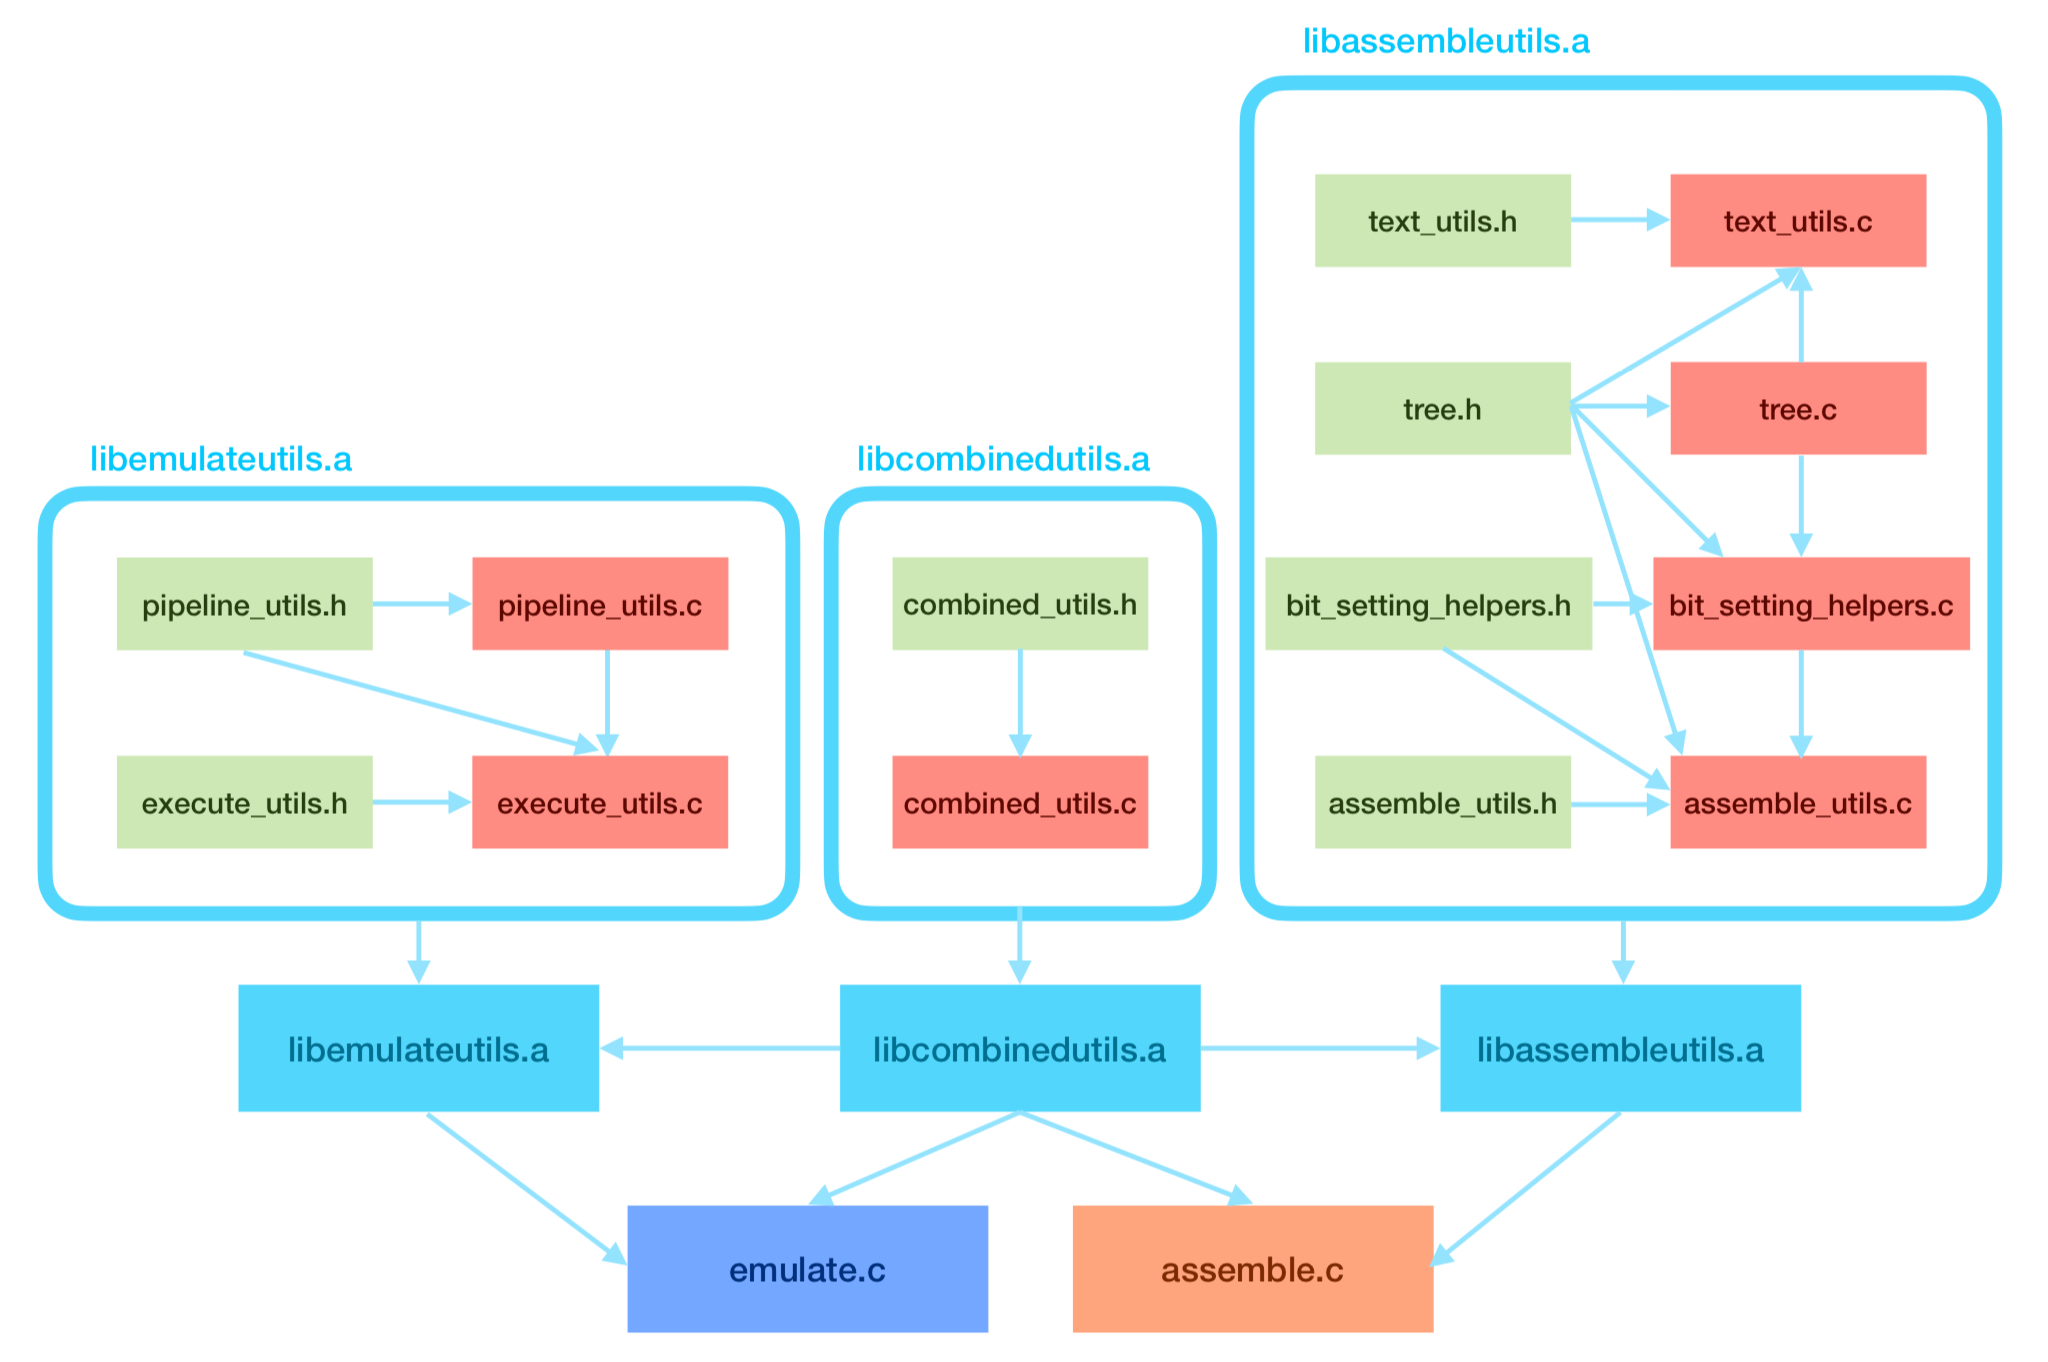
\includegraphics[scale=0.15]{images/emulate_assemble_structure.jpeg}
    \caption{Assembler and Emulator File Structure}
    \label{Figure 1}
\end{figure}

\section{Extension Overview}
We have created a grid-based pandemic spread simulator with a choice of terminal or graphical output in the form of an animated gif. 
The gif output is produced using an open source C gif encoding library \say{Gifenc}, created by Marcel Rodrigues \cite{gifenc}.
The aim of the simulation is to provide a clear and simple demonstration to the average person on how quickly a pandemic can spread and how social distancing and self-isolation can slow the rate of its spread. 
A user can edit the parameters of the simulation such as its chance of infection, grid size and number of humans via a config file before running the simulation. 
The output format can be selected within the application via the terminal: the terminal output providing a step through of a given number of turns printed on the terminal, and the gif output producing a gif of a certain number of turns. The program launches with default values of all variables not found in the config file so the user cannot accidentally break the program.
There is a \say{README} outlining how to use the config file and the colour or alphabetical coding of the respective output format.

\par We believe one of the most impactful features of our simulations compared to others available is the placement of \say{social spaces} across the board, which human agents have a higher chance to move towards using a path finding algorithm. 
The user can control the number of these places across the board and therefore see the direct impact travel and population density has on the spread of the pandemic. 
The user can also decide whether people with symptoms quarantine themselves and whether recovered patients gain immunity to see how these factors also affect the spreading of the pandemic.

\section{Extension Implementation}
 Our extension file structure can be seen in Figure 2, with \say{simulate.c} producing the executable file. 
 The \say{lib} library is used for the general operation of the program and \say{gifoutput} is used to produce the animated gifs. 
 Inside \say{lib} we have files for handling file reading and terminal output (\say{simulationIO}), grid management and updating (\say{simulate\_utils}), and for implementing path finding (\say{simulate\_social.c}).
 \say{Gifoutput} contains the \say{gifenc} library \cite{gifenc} and a \say{gif\_output} file which we use to call the \say{gifenc} functions by translating our programs variables into suitable input for the gif encoder. 
 There are many states of cells on the grid: human cells can be \say{HEALTHY} (uninfected), \say{LATENT} (infected with no symptoms), \say{SICK} (infected with chance to either recover or die) and \say{DEAD}. 
 A grid cell can be \say{NORMAL} or \say{SOCIAL} (making it a \say{social space}, more likely to be moved towards). Cells within a certain range of \say{social spaces} are \say {NEAR\_SOCIAL} and drawn in the same colour as \say{social spaces} to make them more prominent.
 
\par Simulate has a simple structure. It first either reads from the config file or takes default values to initialise the program's variables and then assigns space for the grid on the heap. 
It then creates the humans variable by initialising both a dynamically allocated array of x and y points in the grid that haven't yet been taken up by a human, and an array of human structs. 
A random index is repeatedly selected from the points array and a new human struct is added  to the humans array with a \say{HEALTHY} status and matching coordinates, removing the now taken point from the points array. 
Each human is also initialised with a randomised \say{risk} at this stage, which will determine the chance of them developing symptoms if they are infected. 
Once all humans are placed, a selected few are edited to have \say{LATENT} state and a selected few grid cells are set to have the \say{SOCIAL} state. 
The user enters what input and output they want and the program runs a different simulation loop accordingly. This file also employs a similar error handling system to that used in the assembler to check all dynamic memory allocations and quit, freeing all dynamic data if any processes fail. 
This was necessary since we allocate an amount of data dependant on user input, so we needed to be able to safely handle the scenarios where they ask to assign more memory than they have available.

\par The input loop calls two key functions inside a \say{makeTurn} function: human movement and infection checking. 
The movement function loops through every human and either moves them in a random direction or tries to move them towards a social square using a modified version of the A* algorithm. 
Our path finding algorithm uses more of a greedy approach as every turn it is called it is immediately moved to the neighbouring cell with the lowest heuristic rather than checking a whole path. 
Since the board changes every turn, a path longer than one could be blocked in the next turn. The infection checking algorithm determines whether a \say{HEALTHY} person becomes \say{LATENT}, a \say{LATENT} person becomes \say{HEALTHY} or \say{SICK} and whether a \say{SICK} person becomes \say{DEAD} or recovers to \say{HEALTHY}. 
It loops through every human and examines their status. If they are \say{HEALTHY} it performs a random check for each \say{LATENT} or \say{SICK} person in the eight neighbouring cells, setting their status to \say{LATENT} if any of the checks are successful. 
If they are \say{LATENT}, it reduces their latencyTime by one and sets them to either \say{HEALTHY} or \say{SICK} based on a random check against their risk value if the latency time is 0. 
If they are \say{SICK}, it performs a random check for recovery and death based on the fatality and recovery rates inputted.

\par Outputting to the terminal is achieved by looping through the grid and printing a character based upon either the cell’s human’s status or the cell’s status depending on whether it contains a human or not. 
Creating the gif output is more complex as we had to use a \say{gifenc} handler, which needs the dimensions of the gif and a customised colour palette as well as settings on whether or not to loop the gif and information on the delay between each frame. 
The \say{gif\_output} header contained a function to create the handler with the information of the grid width, height and the size of cells in pixels so the main loop was less congested. 
When adding frames to a gif in \say{gifenc} you populate an array of unsigned integers in the \say{gifenc} handler struct with indexes to colours in its colour palette to draw each pixel. 
Therefore, we made a \say{drawCell} function to draw a single cell given its x and y coordinates, the cell size and its colour and called this for every cell of the grid.
A \say{gifenc} function is called to draw the frame and move forwards by a given delay, which we made a defined constant of 0.1 seconds, after each frame. 
After the turns limit given by the user is reached, a \say{gifenc} library close function is used to close the gif file, creating the gif.

\begin{figure}[t]
    \centering
    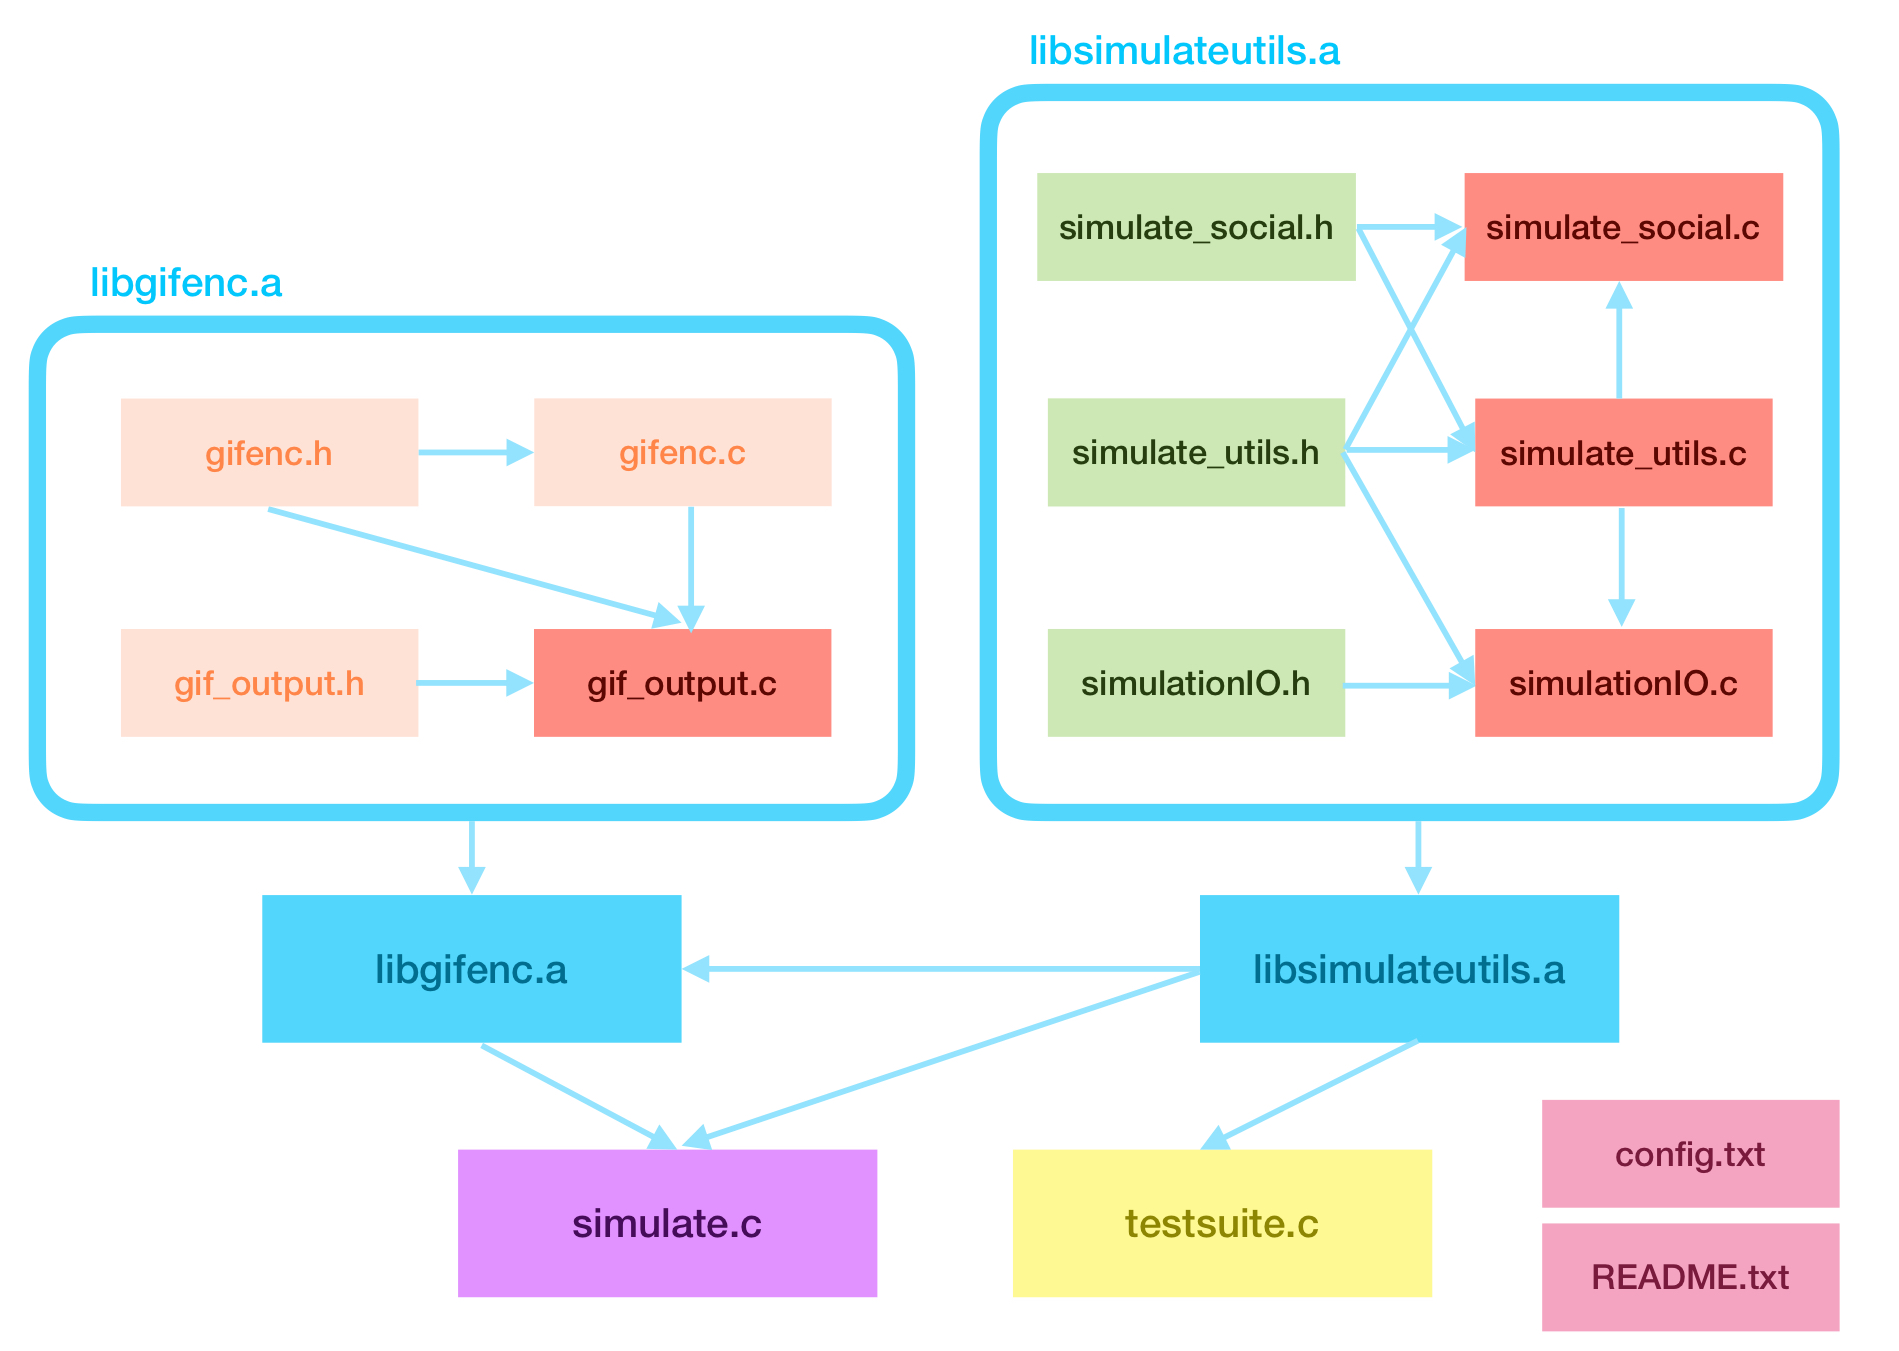
\includegraphics[scale=0.1]{images/extension_structure.jpeg}
    \caption{Extension File Structure}
    \label{Figure 2}
\end{figure}

\section{Extension Testing and Challenges}
 We created a test suite heavily based on the one demonstrated in the programming tools lectures. 
 As our program relies so heavily on randomisation, we ran many of our tests with seeded random values and recorded the results of \say{rand()} for this seed to use when generating our expected values. 
 This test suite was used before every commit to try and ensure there were no bugs in the early stages of development that could go unnoticed. 
 We also used a library called \say{UBSan} to check our code for undefined behaviour to be sure it works on all machines \cite{ubsan}, and  \say{valgrind} to remove memory leaks. 
 We also performed frequent stress testing as we thought execution speed would be a key part in determining the usability of our program. Grids were feasible with up to around 1,000,000 cells in gif mode before execution times started increasing above a minute on our machines. 
 This is because we have taken lots of precautions to only process crucial data such as deleting humans when they die and resizing the humans array so less humans are processed the next turn.
 
\par The first major obstacle we ran into was a fault in the infections algorithm, a bug picked up by the test suite. 
The issue was that humans were processed one by one and therefore if a human was placed next to an initially \say{HEALTHY} cell that had become infected earlier that turn, there was a chance to become \say{LATENT} by the initially \say{HEALTHY} cell. 
This meant it looked like the cell was infected by a \say{LATENT} cell two cells away. We had to overhaul the infections checking to use a new grid of the previous status enums before any changes occurred, so that we could check each human one by one safely without processing incorrect values. 

\par Another problem was found in stress testing when trying to run densely populated grids.
We were initially placing humans randomly in the grid, repeatedly trying new positions until a free one was found.
This made processing dense grids pretty much impossible as to generate a grid of 50 cells, all containing a human would take over $3 * 10^{64}$ random picks on average.
Therefore, we changed the algorithm to create an array of free cells and pick randomly from that array, then removing an element and resizing the array when a human is placed.
This massively improved start up speed and meant it was possible to have simulations with a completely full board.

\par The biggest problem we faced was of our own creation as we named our variables for the rows and columns of the grid \say{gridLength} and \say{gridHeight}. 
This caused much confusion as some people would normally use the terms \say{length} and \say{width} to define a rectangle and others would use \say{width} and \say{height}, so the variables corresponding to columns and rows were inconsistent in the program. 
This eventually caused segmentation faults in many different functions where nonexistent grid cells were being checked and caused the gifs to be drawn in the wrong orientation with a black bar through the middle. 
We eventually renamed these variables \say{gridRows} and \say{gridColumns} to avoid this ambiguity and had to spend much time changing each occurrence of the old names.

\par The result of this testing is that our program is very effective at producing simulations that are visually appealing and get across the points of showing the dangers of high movement and dense population in the spread of a pandemic. 
We think that our program is a very user friendly model as in the terminal output mode you can view thousands of iterations fairly quickly and with the gif output you can produce some visually impressive demonstrations of a pandemic spreading. 
One major pitfall we discovered is that the file size of outputted gifs grows massively with large grids, as the \say{gifenc} library does not use any compression on its gifs, so sometimes gifs can take a long time to load in larger simulations.

\section{Group Reflection on the Project}
For the assembler, we frequently decided to work as individuals but still merged our work in the mornings as we felt that our previous strategy of mainly working as either a group of four or two groups of two was too slow and we that we could maintain code understanding in the group by explaining our changes when merging. 
There were a few sections achieved with pair programming such as the main function in \say{assemble.c} and the insertion and retrieval of data to and from the symbol tree, and when working as individuals we tried to be in a call with at least one other group member to get help.
The approach was fast; we managed to get a skeleton code of all the required functions complete in a few days.
However, we had to spend almost an equal number of days debugging, which almost exclusively had to be done as a group of four, since only one person in the group would know about the piece of code being debugged.
Furthermore, it resulted in a lack of testing during development as we did not have each other’s code to run our functions with, so debugging had to be done in one huge block rather than gradually as we went along.
As a result, we think these collaboration methods were not as effective as those we used in the emulator. 

\par Therefore, in the extension we reverted to frequent use of paired programming to develop the key functions and only used individual programming for hot-fixes or very small tasks like adding error checking.
At the very beginning, we decided that only Matthew and Nicole would work on the extension whilst Izabella and Una continued fixing the assembler, and we managed to produce the first basic prototype with random movement and terminal output by the time the assembler was finished.
Una also developed an initial test suite at this point to ensure we could debug throughout development. 
We then split into teams of two again with Izabella and Matthew implementing gif-based output options and speed optimisations and Nicole and Una implementing the path finding, using the same teams to implement different finishing touches as the deadline drew closer.
These methods of constant team-work and split tasks were the most effective of our entire project, as everyone was constantly kept busy and kept a good understanding of the code structure. 
In addition, we were able to debug simultaneously in smaller groups which drastically improved speed and meant we could add many features to the program.

\section{Individual Reflections}
 \say{We communicated very well as a group and everyone was always ready to help others. 
 I think the approach used in writing the assembler could have been more effective as we had to spend a lot of time going through other people's work to understand it fully.
 Another issue that I struggled with was undefined behaviour as the assembler worked on Linux but would segmentation fault on my Mac. Since we didn’t pass all the tests at that time, we decided that we would leave this undefined behaviour and fix it later which meant that I wasn’t able to run the test suite on my computer.
 The approach we took in the extension was much more efficient. 
 We still had some miscommunications which often led to confusion and we probably could have avoided them  but again we prioritised progress over clarity. 
 Even though we have encountered a fair amount of problems on the way, we always used them as an opportunity to learn and improve.}
\begin{flushright}
- \emph{Izabella}
\end{flushright}
 \say{Personally, I think the group collaborated in a very friendly and professional manner, considering the number of hours we were working daily. 
Everyone was eager to work and willing to give up their time to make the project work. 
I do think that we slowed ourselves down by rushing into the assembler without a clear plan and worked as individuals too often at this stage, resulting in a lot of code that I had never seen before when it was my turn operating the debugger. 
However, I think we resolved these issues when splitting work for the extension as we had a clear timescale and objectives laid out before we began coding. 
Reverting to paired programming massively helped the code understanding in the group and sped up our debugging in this section, whilst keeping a good code writing speed. 
Additionally, I was struggling with an unreliable internet connection throughout the project, so want to thank the team for their patience when I was unable to view the coding stream or join a call.} 
\begin{flushright}
- \emph{Matthew}
\end{flushright}
 \say{Working on this project proved to be not only a pleasant experience but one during which I have learnt a great deal. 
 Group debugging sessions, although quite time consuming, turned out to be very useful as hearing different approaches to a problem helped me to develop a more logical debugging approach. 
 I also enjoyed the pair-programming sessions we had; being able to work with each of my teammates individually meant getting a better understanding of their personal programming style. 
 In the beginning, I found it intimidating writing code which would later be used by my teammates that could lead to bugs if I wasn’t careful enough. 
 Analysing functions on a smaller scale and believing in my abilities helped me overcome this problem by the end of the project. 
 Although starting the C project from the ground up with no previous experience in the language was daunting, it was a very rewarding experience for me. 
 It allowed me to not only improve my communication skills but my programming and debugging skills as well.}
\begin{flushright}
- \emph{Nicole}
\end{flushright}
\say{I felt that the group worked well together, and I enjoyed working with everyone in the team. 
Everyone in the group was helpful and contributed as much as they could to the project. 
Meeting up regularly was really useful, as it meant we were able to delegate jobs efficiently and that everyone was aware of what would be changing in the code at each point in time. 
Merging as a group was also useful as everyone knew when changes were happening to the master branch. 
Having more than one person debugging at a time was also useful as debugging can be a disheartening and strenuous activity alone. 
We used pair programming a lot in the emulator, so tried a more individualistic approach for the assembler, which ended up being faster for code writing, but slowed down debugging. 
The balance we had for the extension worked better, with a mix of the two and a more structured plan going into the project.}
\begin{flushright}
- \emph{Una}
\end{flushright}

\begin{thebibliography}{6}
\bibitem{gifenc}
Rodrigues, Marcel.
"Gifenc"
\texttt{https://github.com/lecram/gifenc}

\bibitem{ubsan}
Clang 11, 
"UndefinedBehaviorSanitiser" \\
\indent \texttt{ https://clang.llvm.org/docs/UndefinedBehaviorSanitizer.html}

\end{thebibliography}


\end{document}